\appendix

\chapter{Spørgeskema}
\label{bil:sporgeskema}
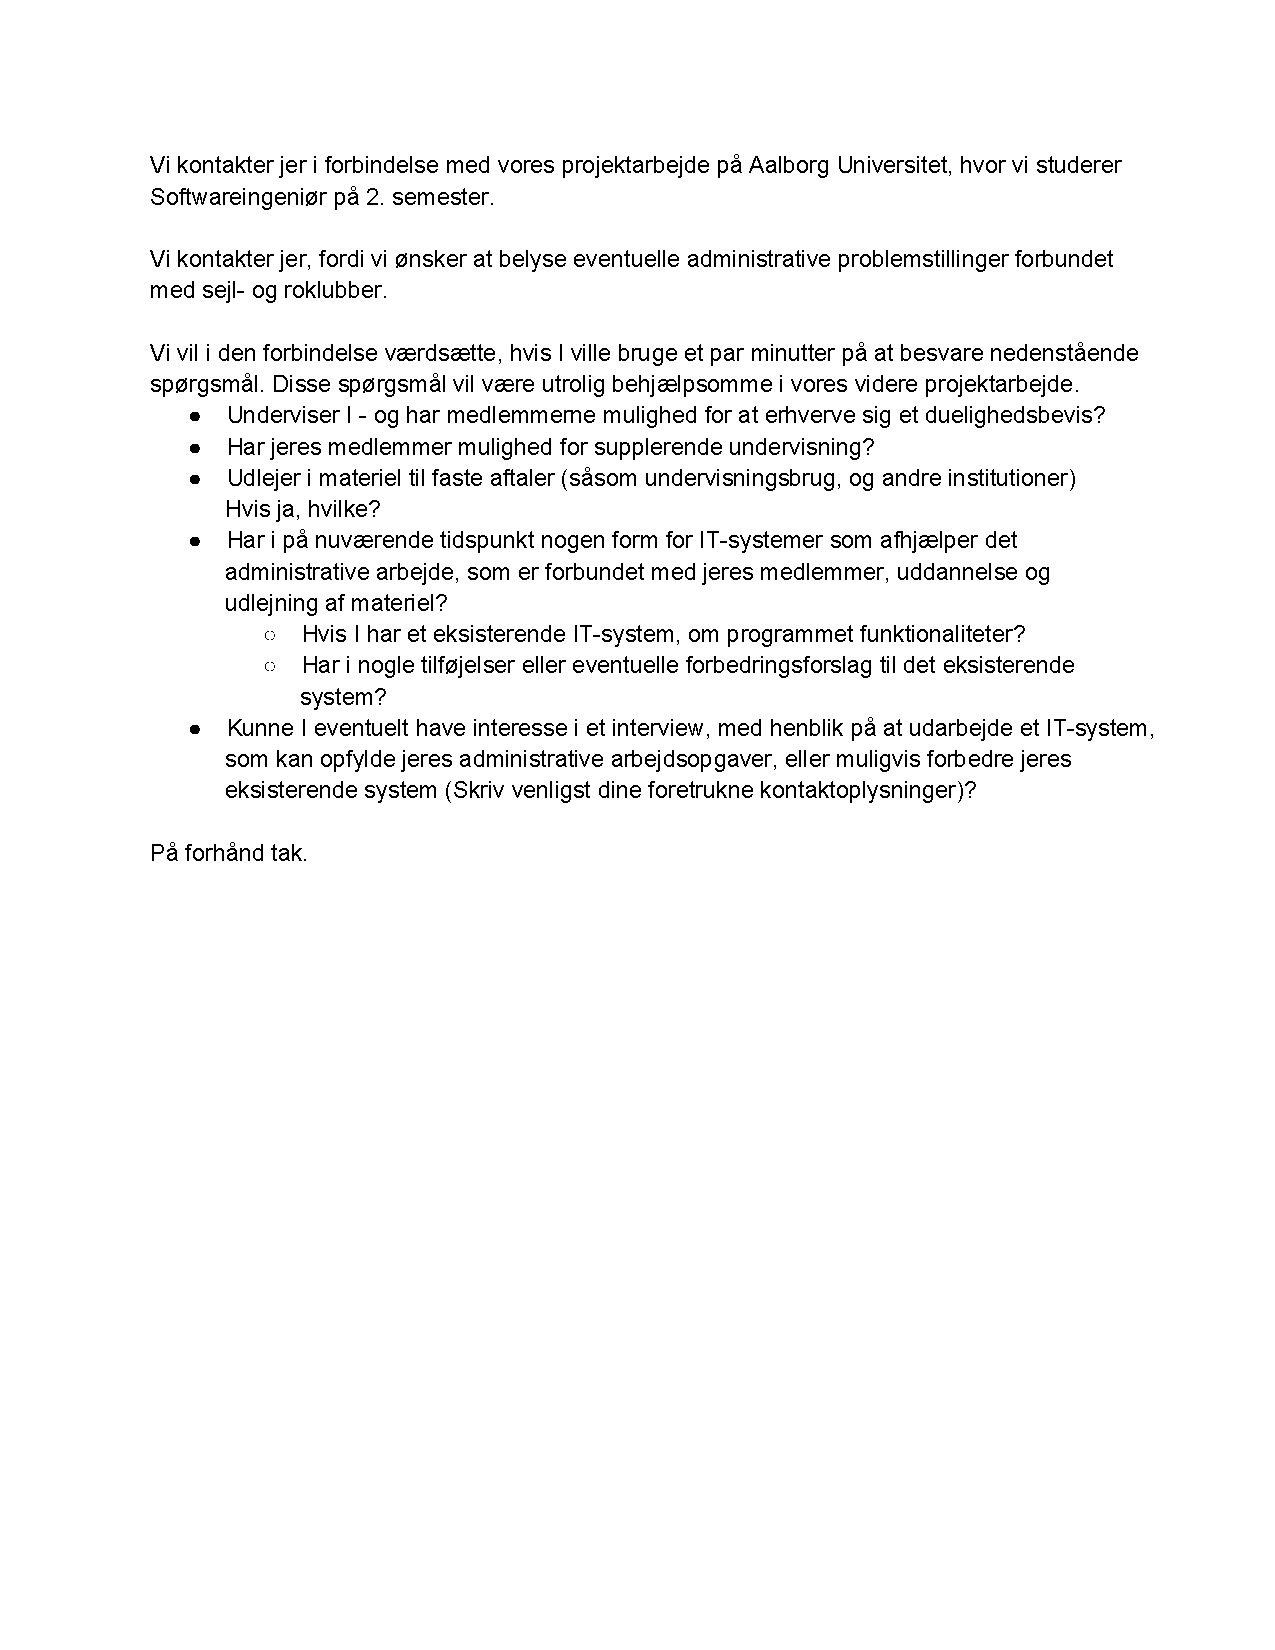
\includepdf[pages={1-}, pagecommand={}]{Kapitler/Bilag/Indledende_Spoergsmaal_Mail.pdf}


\label{FIRSTAPPENDIX}
% Denne skal placers imellem 1. og 2. bilag

\chapter{Interview af Aalborg Roklub}
%Skrevet af Jimmi. 24-02-2014 23:01

\label{bil:interview}
Bilag \ref{bil:interview} indeholder interviewet af Aalborg Roklub. Interviewet foregik mellem Aalborg Roklubs bestyrelsesformand, Karsten Holt og næstformanden, Jens Brandt. Interviewet blev afholdt d. 13-02-2014, kl. 18.00 - kl. 21.00. \\

{\bf Læsevejledning} \\
Spørgsmålene er kategoriseret under 4 overordnede emner. Indledningsvis er der blevet opstillet en række formål, som ene og alene er til gruppens interne brug. Efterfølgende er spørgsmålene opstillet, hvortil respondanternes besvarelser er angivet med kursiv. \\

{\bf Anmærkning} \\
Besvarelserne er blevet tilpasset så de forekommer under de repræsentative spørgsmål. Ydermere er de forklarende besvarelser blevet omskrevet af gruppen. Derfor kan besvarelserne ikke anses som eksakte uddrag fra interviewet. 
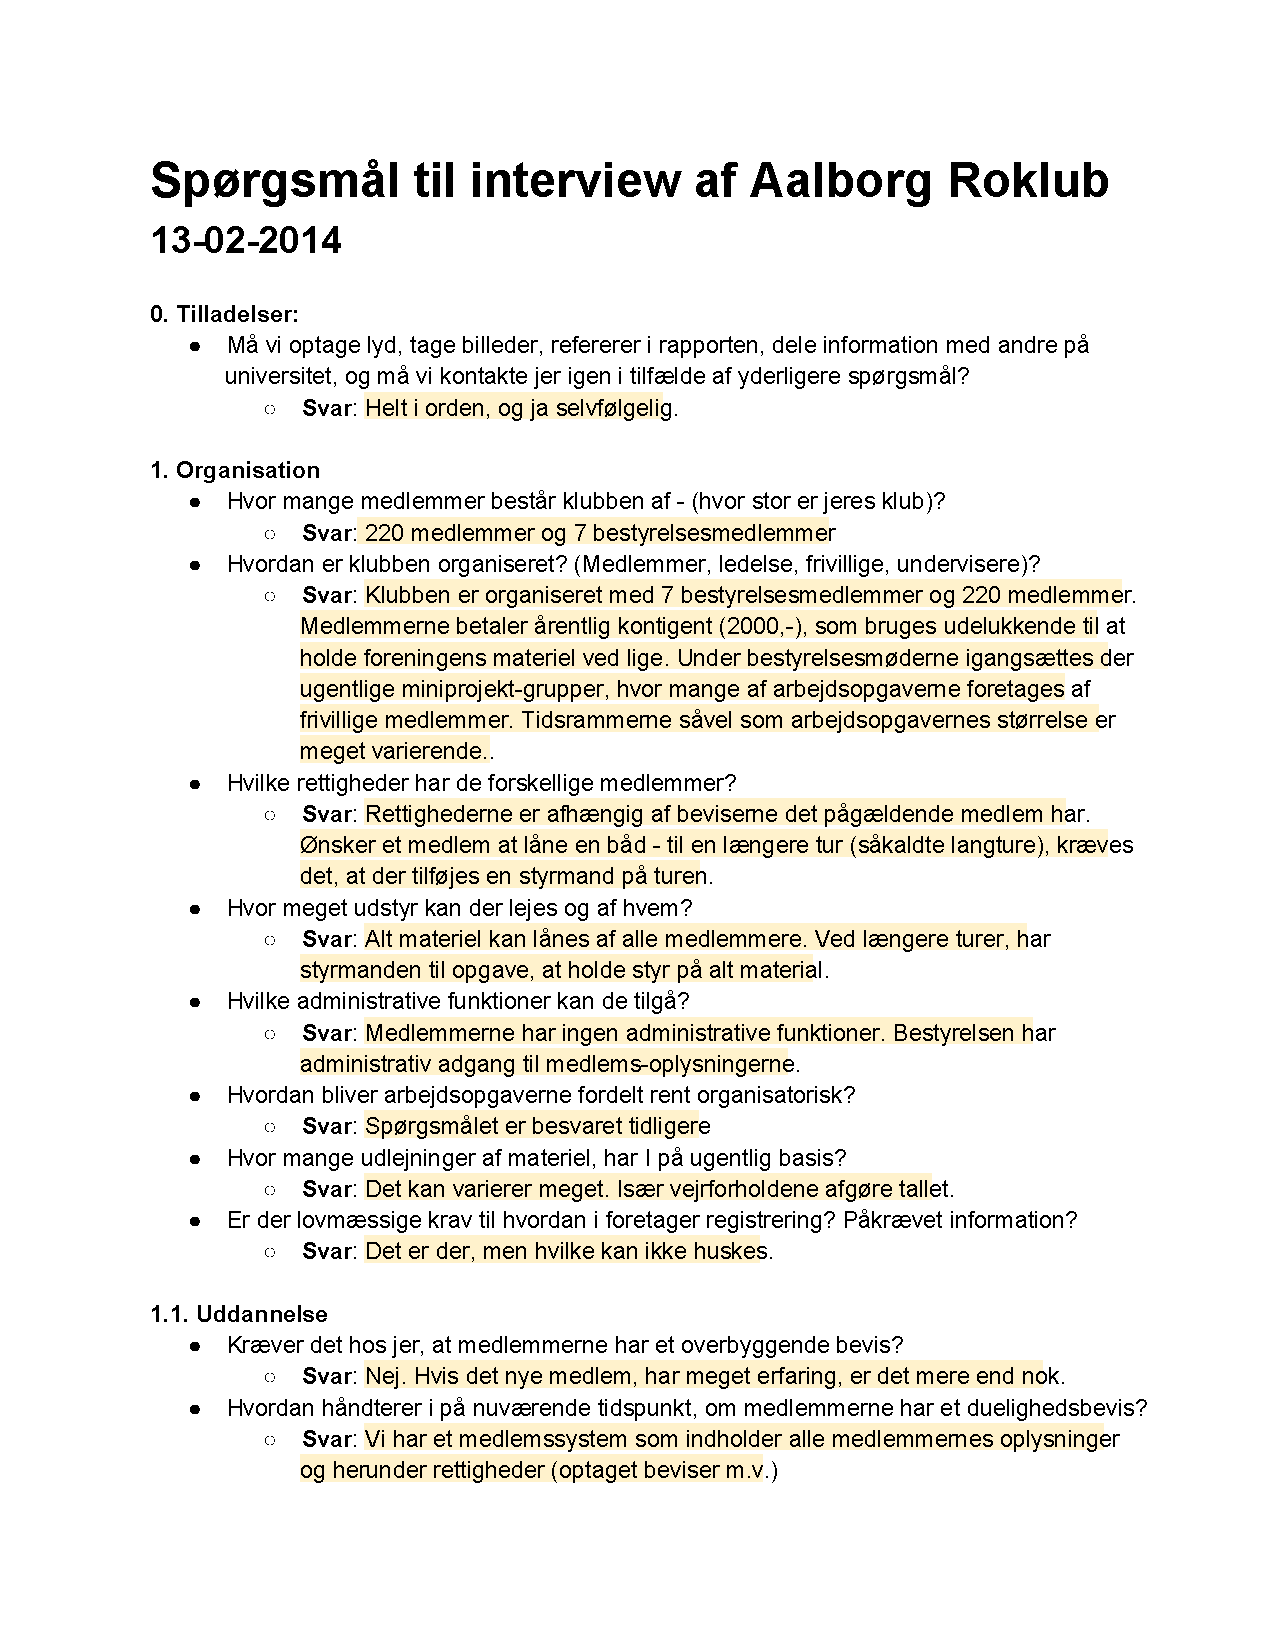
\includepdf[pages={1-}, pagecommand={}]{Kapitler/Bilag/InterviewmedAalborgRoklub.pdf}

\chapter{1. Iteration med Aalborg Roklub}
\label{bil:iteration1}

% Mikkel, 03-05-2014

Bilag \ref{bil:iteration1} indeholder referatet fra 1. iteration med Aalborg Roklub. Interviewet foregik mellem Aalborg Roklubs bestyrelsesformand, Karsten Holt og næstformanden, Jens Brandt. Interviewet blev afholdt d. 18-03-2014.\\

{\bf Anmærkning} \\
Besvarelserne er blevet tilpasset så de forekommer under de repræsentative spørgsmål. Ydermere er de forklarende besvarelser blevet omskrevet af gruppen. Derfor kan besvarelserne ikke anses som eksakte uddrag fra interviewet. 
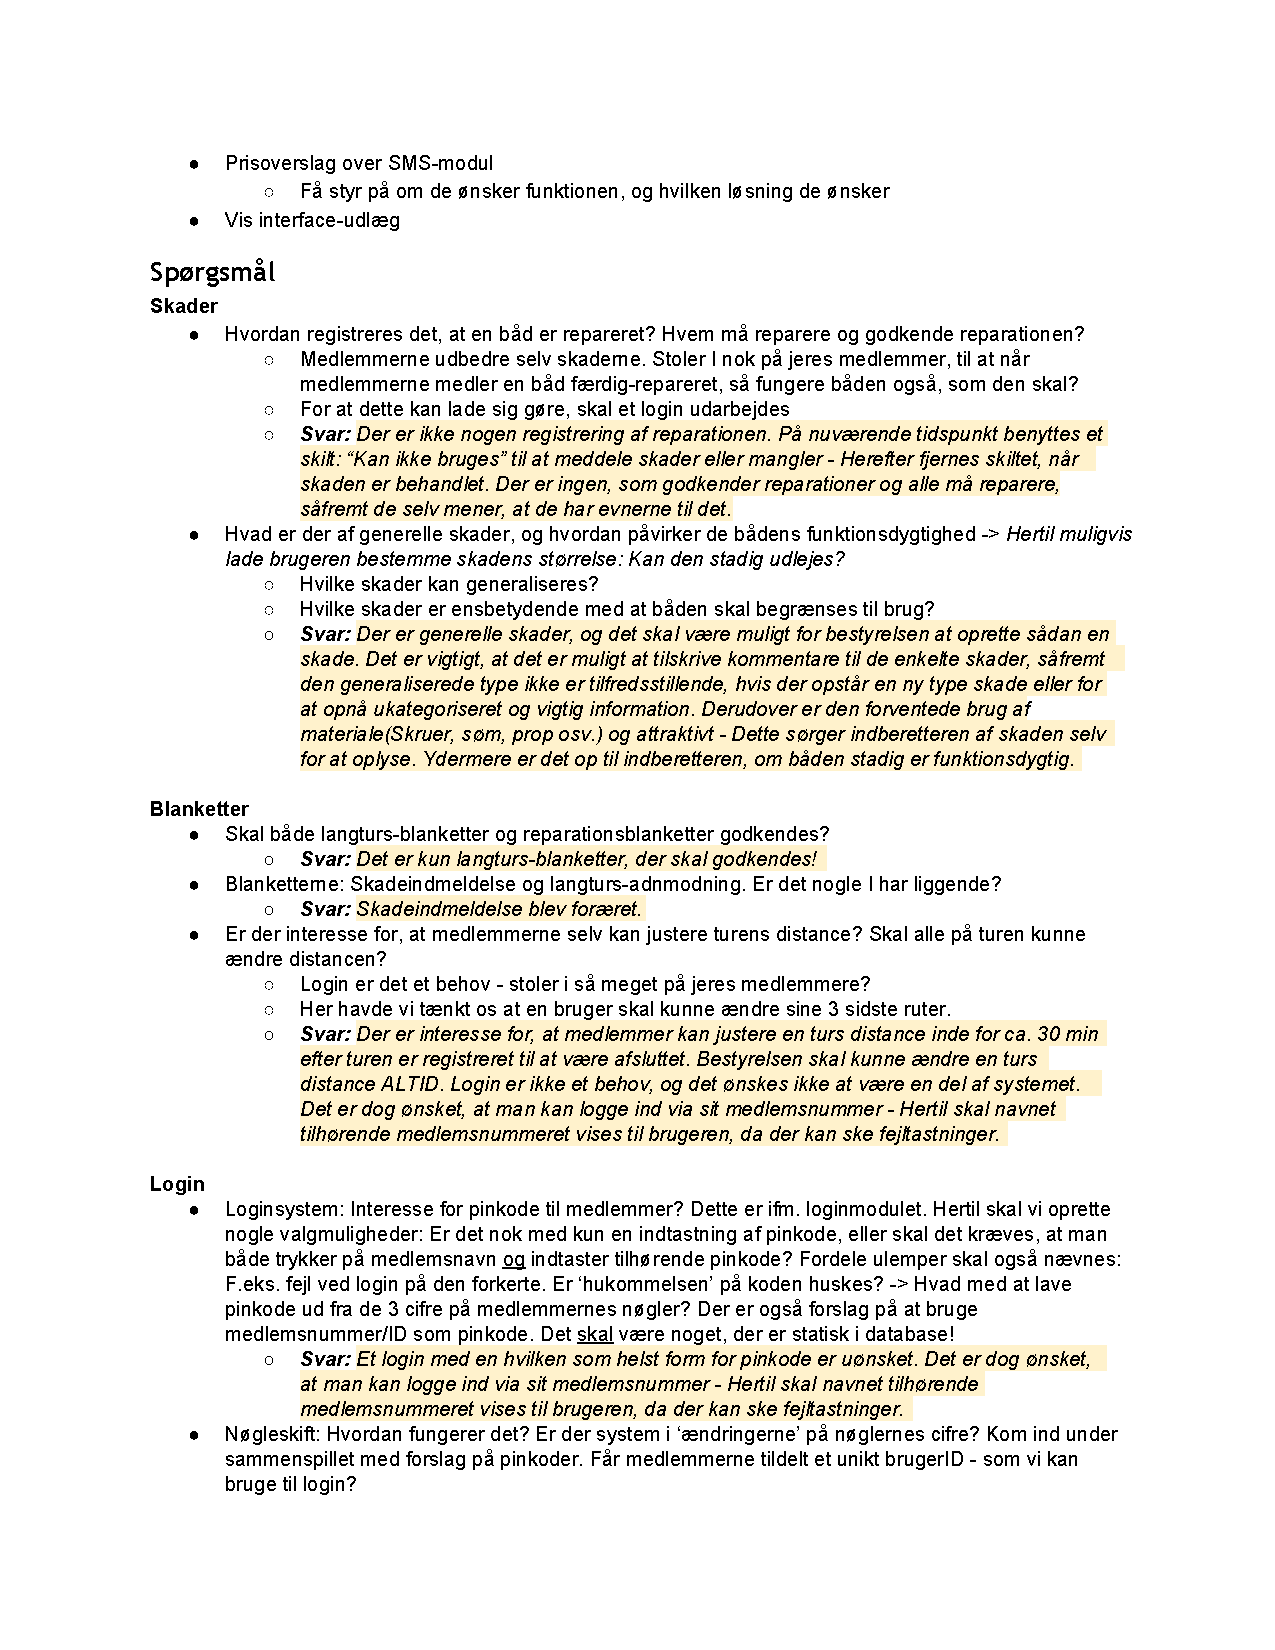
\includepdf[pages={1-}, pagecommand={}]{Kapitler/Bilag/Iterationer/Iteration1.pdf}

\chapter{2. Iteration med Aalborg Roklub}
\label{bil:iteration2}

% Mikkel, 03-05-2014

Bilag \ref{bil:iteration2} indeholder referatet fra 2. iteration med Aalborg Roklub. Interviewet foregik mellem Aalborg Roklubs bestyrelsesformand, Karsten Holt og næstformanden, Jens Brandt. Interviewet blev afholdt d. 01-05-2014.\\

{\bf Anmærkning} \\
Besvarelserne er blevet tilpasset så de forekommer under de repræsentative spørgsmål. Ydermere er de forklarende besvarelser blevet omskrevet af gruppen. Derfor kan besvarelserne ikke anses som eksakte uddrag fra interviewet. 
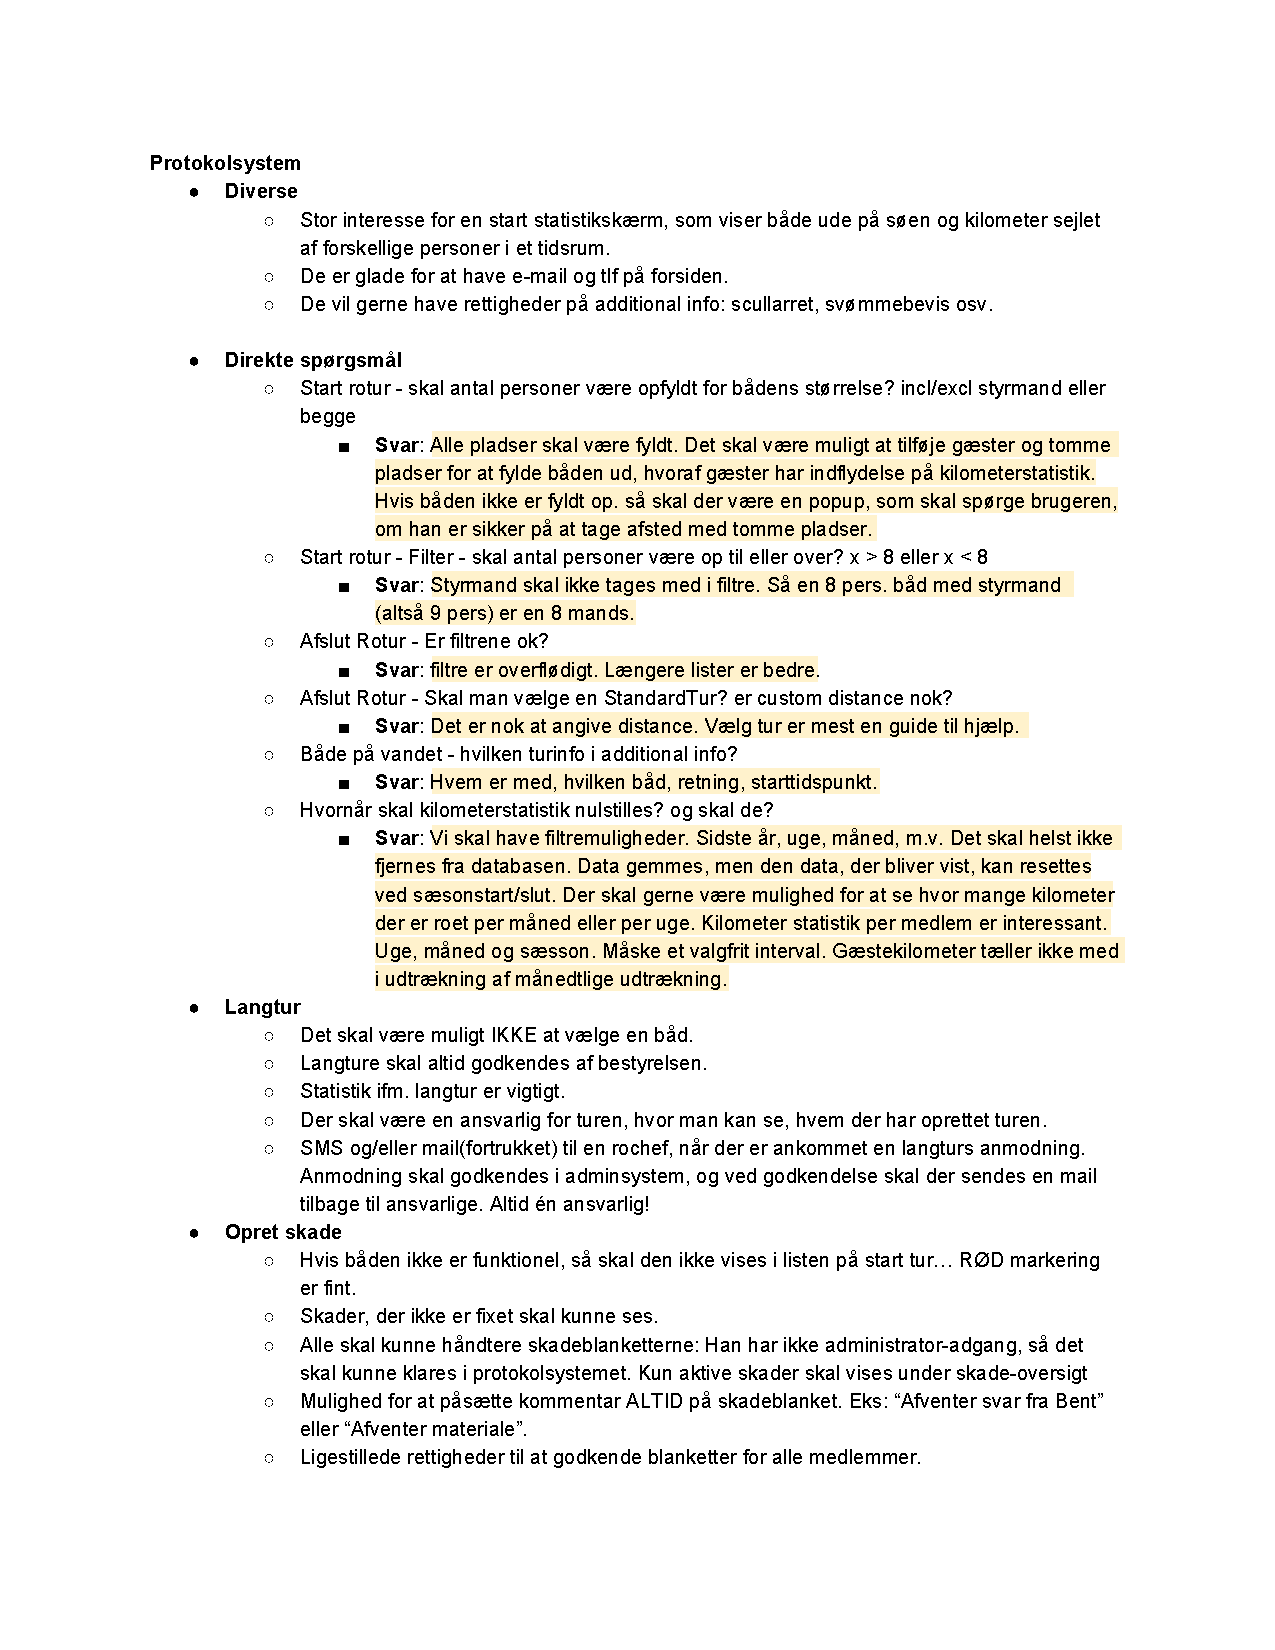
\includepdf[pages={1-}, pagecommand={}]{Kapitler/Bilag/Iterationer/Iteration2.pdf}

\chapter{Aalborg Roklubs skadesanmeldelse}
%Skrevet af Jimmi. 03-03-2014 kl 11:29
\label{bil:ark_skade}

Skadesblanketten er modtaget fra Aalborg Roklub. Denne bruges til daglig i forbindelse med anmeldelser af skader på både.

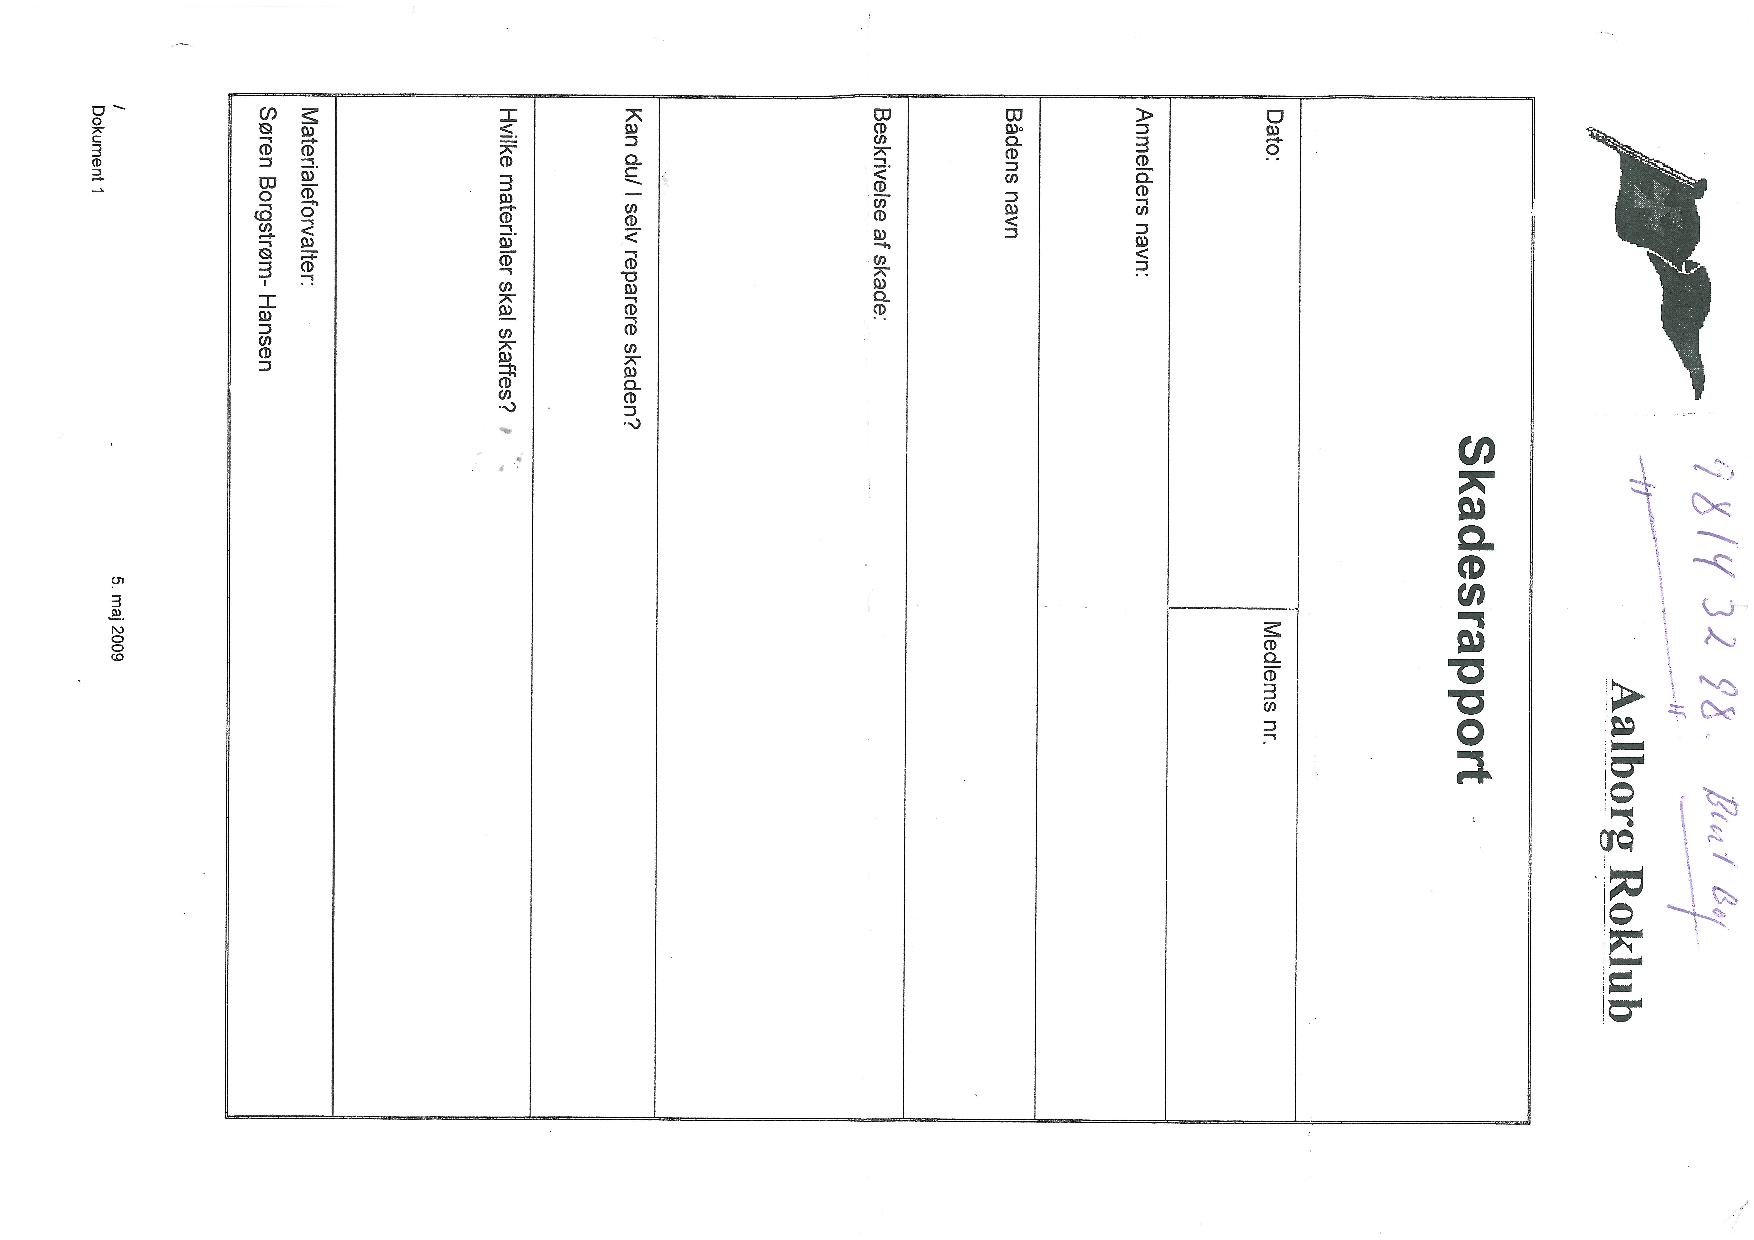
\includepdf[angle=90, pagecommand={}]{Kapitler/Bilag/skadesblanket.pdf}

\chapter{Aalborg Roklubs langtursblanket}
%Skrevet af Jimmi. 03-03-2014 kl 11:29
\label{bil:ark_langtur}
Bilag \ref{bil:ark_langtur} indeholder oplysninger om Aalborg Roklub langtursblanket. Punkterne angivet i bilag \ref{bil:ark_langtur} er uddraget fra en mail-korrespondance mellem gruppen og formanden, Karsten Holt. Korrespondancen blev foretaget d. 3. marts 2014 10:57. \\

{\bf Anmærkning}\\
Oplysningerne er blevet korrigeret, så de indgår i en læsevenlig kontekst. Der er ikke blevet ændret på punktformerne eller ydermere de generelle oplysninger som Aalborg Roklubs formand, Karsten Holt, angav i korrespondacen.

\subsection*{Langtursblankettens indholdsoversigt, skrevet af Karsten Holt}
Ved at studere langtursreglementet fremgår det at flg. oplysninger som minimum skal fremgå af meldingen:
\begin{itemize}
    \item Ansvarlig styrmand for hver båd
    \item Øvrige deltagere
    \item Ønsket båd
    \item Beskrivelse af ruten, herunder dagsdistancer og overnatningssteder
    \item Planlagt afgangs- og hjemkomsttidspunkt
\end{itemize}

Herudover kunne det være vigtigt at flg. oplysninger også fremgik af meldingsblanketten:
\begin{itemize}
    \item Telefonnumre på styrmand og én roer fra hver båd.
    \item I tilfælde af langtur til udlandet at forsikringsforhold på personel og materiel er kontrolleret af styrmanden.
\end{itemize}


\chapter{Sammenligning af værktøjer til klubadministration}
\label{bil:nuvaerende_systemer}


Bilag \ref{bil:nuvaerende_systemer} indeholder det spreadsheet der blev udarbejdet i forbindelse med modulanalysen, hvor allerede eksisterende systemer blev analyseret.\\

{\bf Anmærkning} \\
Følgende bilag er anvendt som arbejdsmateriale til gruppen, hvilket betyder det ikke er udarbejdet på en flot grafisk måde.\\
Systemerne angivet med grøn, er de valgte systemer i modulanalysen.\\

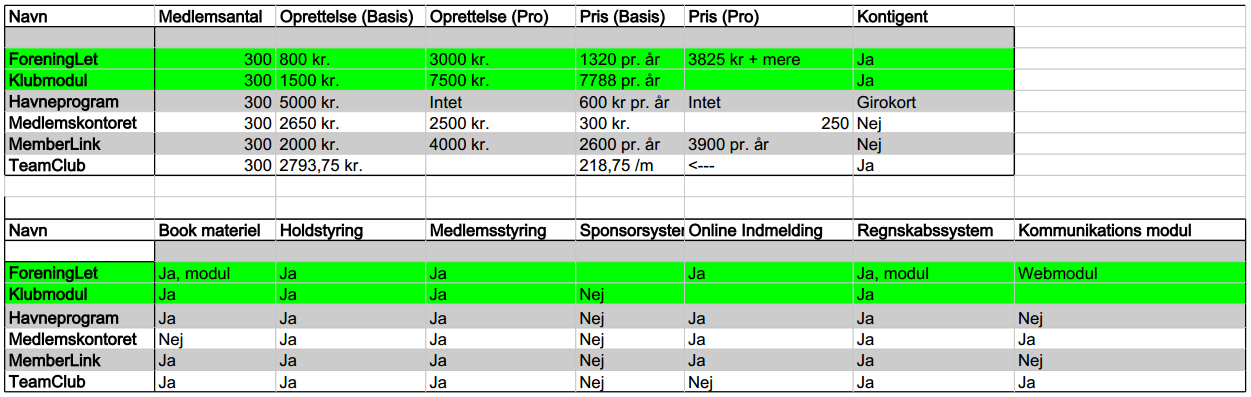
\includegraphics[scale=0.5]{Kapitler/Bilag/sammenligning.png}

%\chapter{Databaserelationer}
%\label{bil:db_relationer}

Dette bilag indeholder relationer i databasen - tabeller uden relationer er fjernet fra figuren.

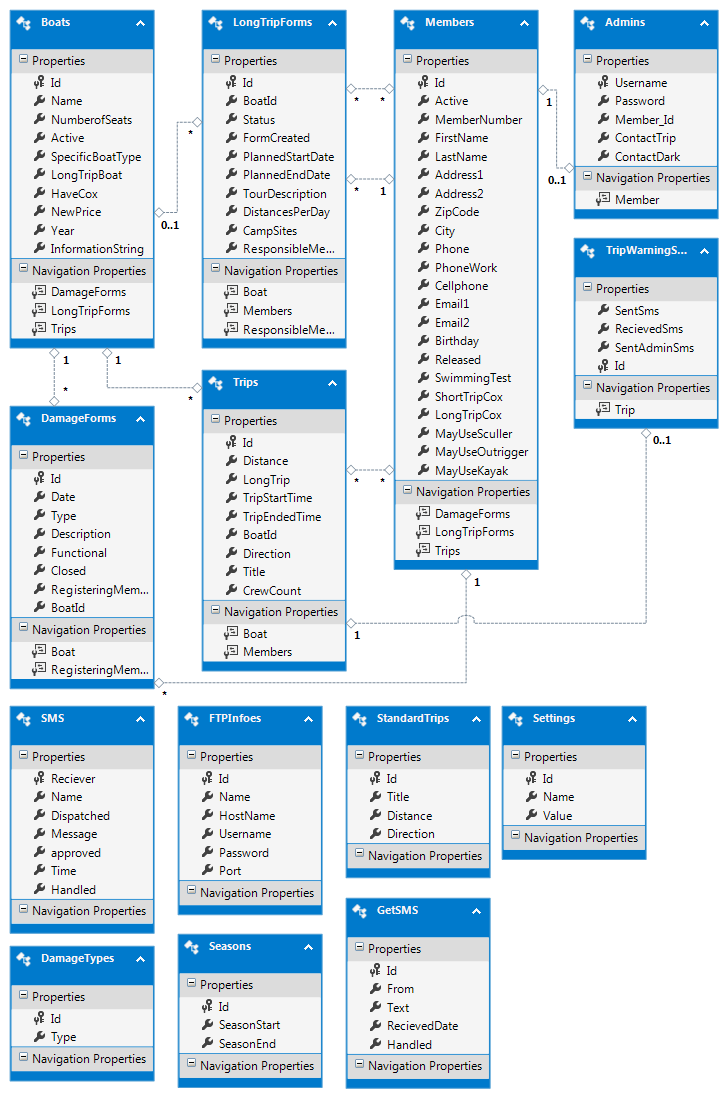
\includepdf[angle=270, pagecommand={}]{Figurer/Database_Relationer.png}

\chapter{Email-korrespondance}
\label{bil:email}
I projektet har det været yderst essentielt at få svar på givende spørgsmål, som er opstået under udviklingsforløbet.
Hertil har gruppen haft en del email korrespondancer, hvor et udpluk af de vigtigeste er medtaget herunder\\
\\
{\textbf{Email-korrespondance (Spørgsmål) fra gruppen}}\\
Hej Karsten og Jens,\\
\\
Vi har lige et par spørgsmål til programmet.\\
\\
Skal styremanden på en tur, tælle med i kilometer-statistikkerne. Både de overordnede kilometre, såvel som de individuelle kilometre?\\
\\
I jeres båd-XML: \\
- I har en property som hedder 'Aktiv' - hvad bruger i denne til?\\
- Hvad bruger i jeres 'bådtype'-property til?\\
\\
Har i mulighed for at vi kan sætte MySQL op på jeres lokale server, således at man også kan tilgå daten udefra?\\

-- \\
Med venlig hilsen\\
Jimmi Nielsen\\
Gruppe: SW2A304, AAU, Softwareingeniør\\
Lokale: A304 \\
Mail: jiniel13@student.aau.dk\\

{\textbf{Email-korrespondance (svar) fa Aalborg Roklub}}\\
Hej Jimmi\\

{\textbf{Styrmænd:}}\\
Styrmænd tæller med på lige fod med alle andre i båden.\\
Specielt i inriggerne byttes der rundt under ro turen, så man kan ikke sådan pille dem ud \\

{\textbf{Båd-XML}}\\
Aktiv:
\begin{enumerate_small}
    \item Båden er i Aktiv tjeneste og kan anvendes
    \item Båden findes ikke i klubben længere – kan ikke anvendes
\end{enumerate_small}

{\textbf{BådType:}
\begin{enumerate_small}
    \item Robåd
    \item Kajak
    \item Ergometer
\end{enumerate_small}
På nuværende systems forside kan man vælge at filtrere på de tre typer.\\

{\textbf{MySQL}}\\
Vi har i dag 5 databaser hos surftown – det bruges af de forskellige systemer vi anvender på web delen.
Vi anvender sådan set alle fem databaser. Der er dog en ’sandbox’, som bruges til at afprøve større ændringer i vores wordpress.\\

Hvis det kun er til noget test, kan i sagtens låne den.\\
Når det bliver permanent, må vi finde ud af at rykker de andre systemer sammen, så der bliver plads til jeres database.
Det burde kunne lade sig gøre.\\
https://phpmyadmin.surftown.com/index.php\\
user: \hl{(Slettet, red.)}\\
pwd : \hl{(Slettet, red.)}\\
servervalg: \hl{(Slettet, red.)}\\
\\
jeg har mulighed for at give adgang ekstern databaseadgang. Jeg skal blot registrere den IP adresse der skal have adgang.\\
 
Mvh. Jens Brandt




\chapter{Usability test}
\label{bil:usability}

\textbf{1. Testcase (Start rotur)}: Du skal starte en ny rotur, med nedenstående oplysninger:\\

Båden du ønsker at leje er: Laubek\\ 
Tilføj en besætning bestående af: 1 styrmand, 2 medlemmer, 2 gæster.\\
Vælg en retning: Øst\\

\textbf{2. Testcase (Afslut rotur)}: Du skal afslutte en rotur, som du lige er kommet hjem fra:\\

Båden du har benyttet er: Laubek\\
Vælg Standard tur: Nordbroen\\
Ændre distancen til 12 km\\

2.1 Testcase (ændre distance): Du har tastet en forkert distance, du ønsker derfor at ændre distancen til 15 km. Gør dette\\

\textbf{3. Testcase (Både på vandet)}: Mørket melder sig på, du ønsker at undersøge hvilke både der ikke er kommet hjem. Gør dette.\\

3.1 Testcase (besætning): Find ud af hvilken besætning den første båd i listen har.\\
3.2 Testcase (telefon-nummer): Find telefonnummeret på det første besætningsmedlem i båden.\\


\textbf{4. Testcase (Opret skade)}: Du er lige kommet hjem fra en rotur i båden Laubek. Du kom uheldigvis til at beskadige båden, så den ikke længere er anvendelig.\\

Skadetype: Skroget er blevet skævt.\\

\textbf{5. Testcase (Opret langtur)}: Du ønsker at tage på en langtur, og vil derfor gerne anmode om dette:\\

Til turen, ønsker du at reservere båden: Kap 71\\

Du ved på nuværende tidspunkt ikke hvilke besætningsmedlemmer der skal med på langturen, men vil stadig gerne anmode om langturen. Udfyld besætning.\\

Du ønsker at tage afsted d. 21-05-2014\\
Du forventer at komme tilbage d. 28-05-2014\\
Du forventer at overnatte i Nibe og Løgstør\\
Dine forventede dagsdistancer er 50 km\\
Din beskrivelse af langturen skal være: Hyggetur\\
Du skal vælge dig selv som ansvarlig
%\chapter{Løsningsforslag (Statusseminar)}
%\label{bil:loesningsforslag_statusseminar}
%\begin{itemize_small}

\item Den lokale database skal tilgængeliggøres fra internettet, således at administration kan ske hjemmefra, enten igennem et installeret program eller en internet-browser

\item Aalborg Roklubs nuværende design sætter en række udbyggelsesmæssige begrænsninger, og derfor forslås det, at der konstrueres et helt nyt bruger-interface (WPF baseret)
\begin{itemize_small}
\item Hertil ønsker vi at sætte speciel meget fokus på interaktionen mellem bruger og system. Dette betyder, at designet vil blive konstruereret på baggrund af velovervejede forudsætninger
\end{itemize_small}

\item Sikkerhedsmæssige aspekter, i form af et SMS-system som underretter bestyrelsesmedlemmer, hvis medlemmerne ikke er kommet tilbage inden mørkets frembrud, eller har været ude meget længere tid end de angav
\begin{itemize_small}
\item Disse tider vil blive reguleret automatisk
\end{itemize_small}

\item En status på udlejningsmateriel, så medlemmerne og administrationen altid kan se bådenes status (om de er ude, hjemme eller beskadiget). Materiel der er klar til udlejning, skal angives som grønne, og beskadiget materiel, skal angives som røde - og derved ikke gøres tilgængelige for andre medlemmer
\begin{itemize_small}
\item Medlemmer skal selv have mulighed for at ændre i bådenes status og beskadigelsestilstand. Hvis et medlem angiver at båden er beskadiget i en sådan grad, bliver et bestyrelsesmedlem notificeret
\item Medlemmerne har kun mulighed for at leje materiel som ikke er registreret som "udlånt" eller "beskadiget"
\end{itemize_small}

\item Ved længere ture - hvor en styrmand er påkrævet - påkræves der af registranten, at der tilføjes et medlem med styrmands-rettigheder til turen. Dette kræver at databasen indeholder informationer om medlemmernes rettigheder (som skal hentes fra "medlemssystemet")

\item Ved hjemkomst skal medlemmerne have mulighed for følgende:
\begin{itemize_small}
\item Juster kilometerne på deres egne ture
\item I tilfælde af skader, skal medlemmerne have mulighed for at indregistrer skadeindmeldelsen elektronisk
\end{itemize_small}

\item Bestyrelsen skal kunne se, hvem der angivet skadeanmeldelserne, ændret bådens status, samt følge op på diverse materiel.
\begin{itemize_small}
\item For at øge logfilens pålidelighed, ønsker vi at konstruere et pinkode login-system (fire tal), til at identificere registranten
\item Et log-system kunne sættes op, så det automatisk kan ses, hvilket medlem der har foretaget registrationen. Med dette system, kunne det være muligt for medlemmer at ændre i alle tur-informationer, samt skadestilstande for materiel (hvis de selv vil reparere skaden eller lign.)
\end{itemize_small}

\item En integrering af medlemsdatabasen fra "medlemssystemet", således at det kun er nødvendigt at indtaste og ændre medlemsdata ét sted

\end{itemize_small}


%Løsningen vil fungere som en viderebyggelse af Aalborg Roklubs eksisterende udlejningssystem (også kaldet protokolsystem). Dette bunder i manglen på en administrativ vinkel i det system, hvor man i dag skal gå manuelt ind i XML-filerne og se hvad der er sket. I det nye system skal det være muligt for bestyrelsen (eller andre administrative organer) at kunne se status og statistik over forskellige ting - her kan blandt andet nævnes hvem der laver flest skader og hvilke både der ikke kommer hjem til tiden. \\

%Hermed fører det over til en logiske sammenkobling i forhold til det sikkerhedsmæssige perspektiv, hvor det er muligt at opstille en kontrol for om nogle af bådene ikke er hjemme efter mørkets frembud (hvilket er et krav i roklubben) - er dette tilfældet, kan det vise sig som et “alarmflag”, hvor styrmanden på den pågældende båd skal bekræfte at alt er under kontrol. Modtager man ikke den bekræftelse, skal et bestyrelsesmedlem alarmeres, som kan sikre sig at der ikke er sket noget med båden eller besætningen.\\

%Af de datalogiske emner vil der blive fokuseret meget på databaser og brugergrænseflader på den måde at der skal laves en databaser over alle båder, deres ruter, anvendelsestidspunkt, skader og så videre. Dette skal stilles op på en god og effektiv måde i en online database (fx ved brug af MySQL), så den kan tilgås overalt, men også så forskellige systemer kan snakke sammen over den samme database. Dette vil blive lavet i C\# mens det nuværende system er i Visual Basic - dette vil dog ikke være noget problem, når der laves en database som begge system kan kommunikere med.
% Slettet af Mikkel, da statusseminar er slut

\chapter{CD}
\label{bil:cd}

Vedlagt på cd-rom:
\begin{itemize}
    \item Program.zip
    \item Rapport.pdf
    \item Flowchart.png
    \item UML-diagram.png
\end{itemize}




\label{LASTAPPENDIX}
% Denne skal placeres til allersidst